A separable allocator is used to handle the case where multiple requesters compete for multiple resources. Instead of performing one large global arbitration, the allocation problem is divided into two simpler arbitration steps. This reduces hardware complexity and makes the allocator easier to pipeline and implement in RTL.

The allocator uses a separable input-first allocation strategy. The requesters are first grouped by input side. In the first arbitration step, each input side selects at most one candidate request from all its active requests. This means that one input can only forward one request to the second arbitration step in a given cycle. In the second step, each resource arbitrates among the candidate requests that target it and selects one final winner.

The overall organization of the separable input-first allocator is shown in Figure~\ref{fig:separable_input_first_allocation}. In this router, the separable input-first allocator operates on the requests from the virtual channels of five input ports. In the first level, each input-side arbiter selects at most one requesting virtual channel from the local VCs of the same input port. This produces one candidate request per input port. In the second level, the selected candidates are grouped according to their target output ports. Each output-side arbiter then selects one winning input among the candidates requesting the same output port. Since the router has five output ports, this stage ensures that each output port accepts at most one input in one cycle. Finally, the selected winners are mapped back to the original virtual channels to generate the final grant signals. In this way, the allocator guarantees that each input port grants at most one VC and each output port is assigned to at most one input.

\begin{figure}[htbp]
    \centering
    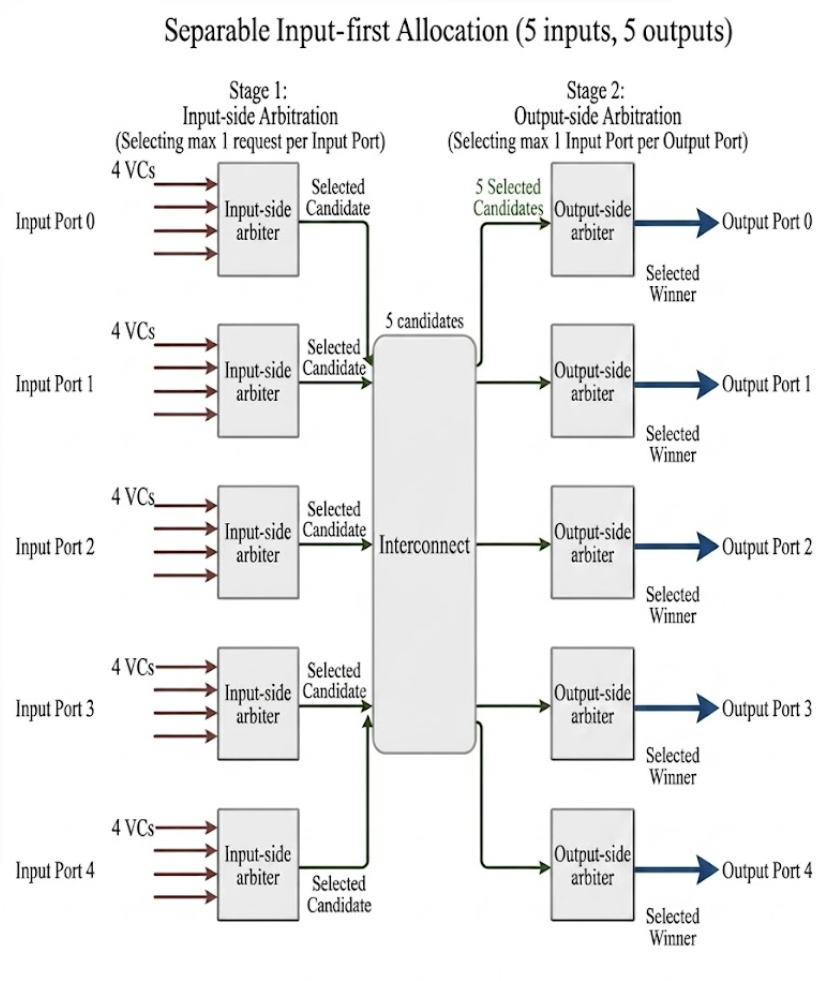
\includegraphics[width=0.8\textwidth]{images/ch3_design_and_implementation/Separable_Input_first_Allocation.png}
    \caption{Separable input-first allocation structure}
    \label{fig:separable_input_first_allocation}
\end{figure}

Figure~\ref{fig:separable_input_first_example} illustrates an example of separable input-first allocation with five inputs and five output resources. In Figure~\ref{fig:separable_input_first_example}(a), the request matrix shows all active requests before arbitration. After the first-stage input-side arbitration, each input keeps at most one selected request, forming the intermediate matrix shown in Figure~\ref{fig:separable_input_first_example}(b). The second-stage output-side arbitration then resolves conflicts among requests targeting the same output resource, and the final grant matrix is shown in Figure~\ref{fig:separable_input_first_example}(c). The final grant matrix contains only conflict-free grants, where each input receives at most one resource and each resource is assigned to at most one input.

\begin{figure}[htbp]
    \centering
    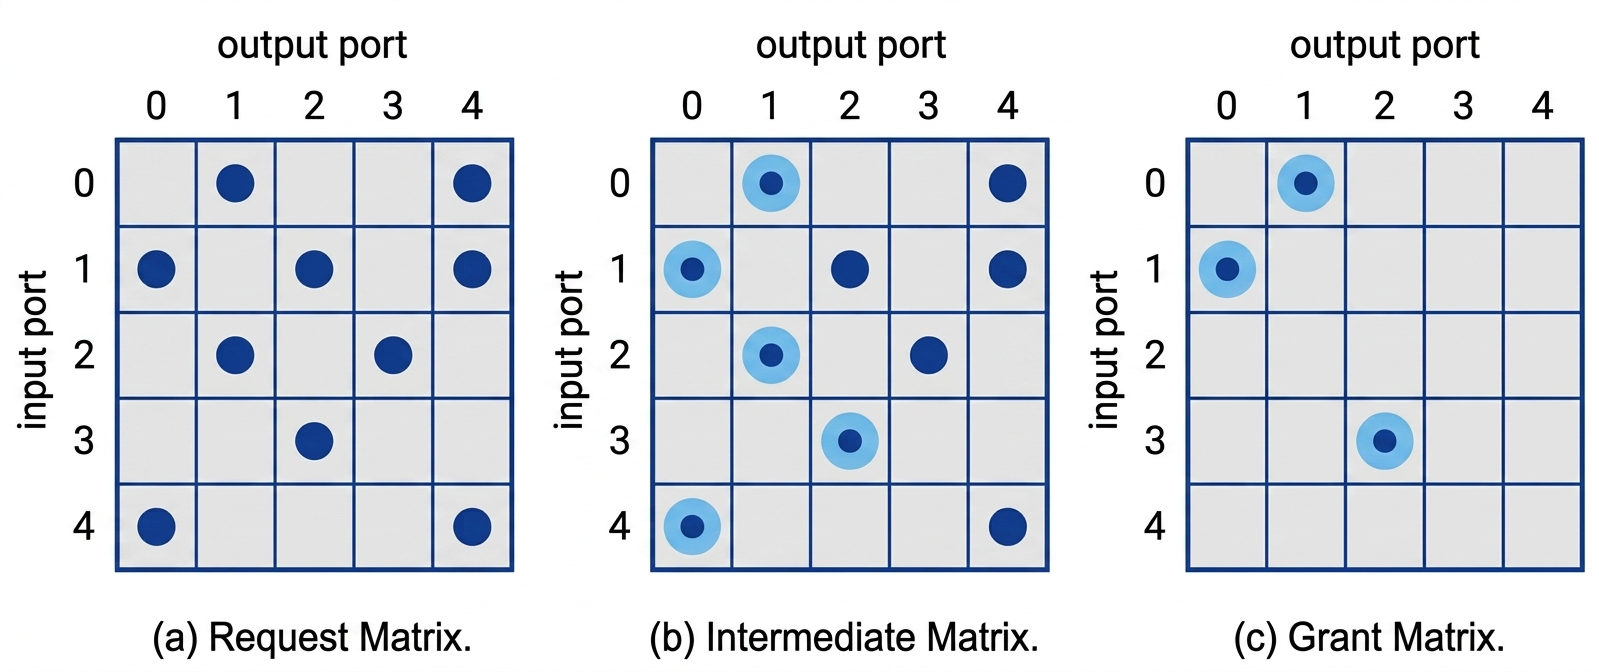
\includegraphics[width=0.9\textwidth]{images/ch3_design_and_implementation/matrix.png}
    \caption{Example of separable input-first allocation.}
    \label{fig:separable_input_first_example}
\end{figure}

The allocation result must still satisfy the basic matching rules: one requester can receive at most one grant, and one resource can be granted to at most one requester. Therefore, the final output of the allocator is a conflict-free grant result.

This approach is suitable for the router design because both virtual-channel allocation and switch allocation involve many requesters and multiple possible resources. By decomposing the allocation into two stages, the design avoids a large centralized allocator and keeps the arbitration logic relatively simple. The drawback is that separable input-first allocation may not always generate the maximum possible number of grants, because the first-stage arbiters make local decisions without knowing the final result of the second stage. However, this trade-off is acceptable for this design, since the main goal is to keep the router simple, predictable, and hardware-efficient.